\documentclass[border=4pt]{standalone}
\usepackage{tikz}
\usetikzlibrary{arrows.meta}
\begin{document}
% ==== Paper 2 (TMLR) cycle schematic -- DISTINCT version of the Part I figure ====
% Same layout, meaning, and axes as Part I, but made visibly distinct by (a) nudging each stage
% node (recruit UP, explore UP+INWARD, consume DOWN, blocked INWARD) and (b) a NEW colour scheme
% (teal / blue / orange / red instead of grey / blue / green / red). Stage labels enlarged
% and bolded for readability. All labels stay upright with the same meaning.
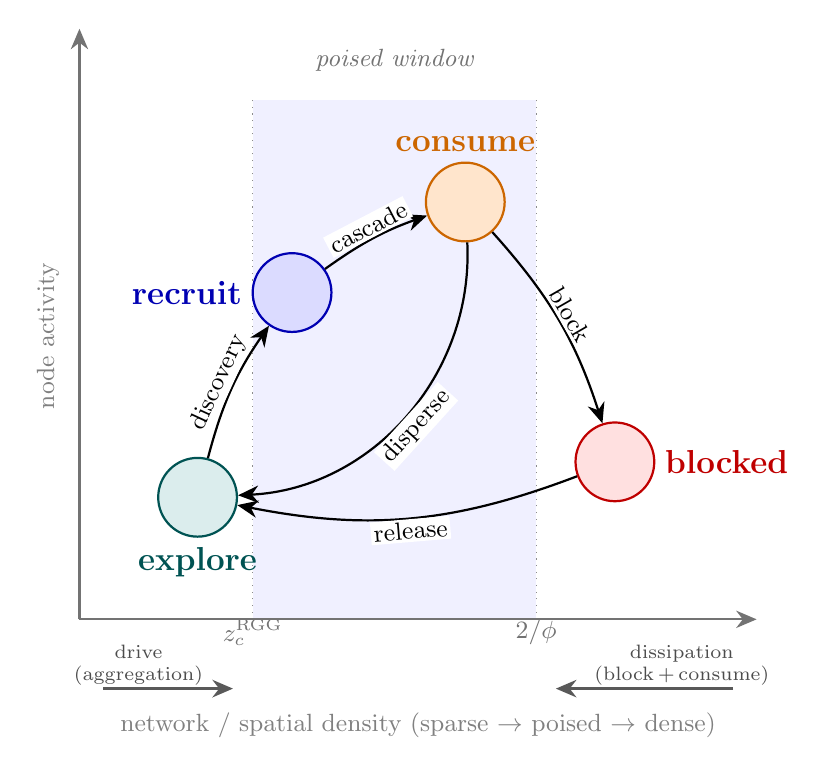
\begin{tikzpicture}[>={Stealth[length=2.6mm,width=2.2mm]},
    E/.style={circle,draw=teal!65!black,fill=teal!14,thick,minimum size=1.0cm,inner sep=0pt},
    R/.style={circle,draw=blue!70!black,fill=blue!14,thick,minimum size=1.0cm,inner sep=0pt},
    C/.style={circle,draw=orange!80!black,fill=orange!20,thick,minimum size=1.0cm,inner sep=0pt},
    D/.style={circle,draw=red!75!black,fill=red!12,thick,minimum size=1.0cm,inner sep=0pt},
    tl/.style={font=\small,fill=white,inner sep=1pt}]
  \fill[blue!6] (4.6,1.3) rectangle (8.2,7.9);
  \draw[black!45,dotted] (4.6,1.3)--(4.6,7.9);
  \draw[black!45,dotted] (8.2,1.3)--(8.2,7.9);
  \node[font=\small\itshape,black!55] at (6.4,8.4) {poised window};
  \node[font=\small,black!55] at (4.6,1.13) {$z_c^{\mathrm{RGG}}$};
  \node[font=\small,black!55] at (8.2,1.13) {$2/\phi$};
  \draw[->,black!55,thick] (2.4,1.3)--(11.0,1.3);
  \draw[->,black!55,thick] (2.4,1.3)--(2.4,8.8);
  \node[font=\small,black!50,rotate=90] at (2.0,4.9) {node activity};
  % ---- stage nodes: nudged from Part I (explore up+inward, recruit up, consume down, blocked inward) ----
  \node[E] (E) at (3.9,2.85) {};   % explore: up + inward toward centre
  \node[R] (R) at (5.1,5.45) {};   % recruit: up, moved left to give the "cascade" edge label room
  \node[C] (C) at (7.3,6.60) {};   % consume: down
  \node[D] (D) at (9.2,3.30) {};   % blocked: inward (toward centre)
  % ---- stage labels: larger + bold, coloured to match the new scheme ----
  \node[font=\large\bfseries,teal!65!black,anchor=north]    at (E.south) {explore};
  \node[font=\large\bfseries,blue!70!black,anchor=east]   at (R.west)  {recruit};
  \node[font=\large\bfseries,orange!80!black,anchor=south]  at (C.north) {consume};
  \node[font=\large\bfseries,red!75!black,anchor=west]  at (D.east)  {blocked};
  \draw[->,thick] (E) to[bend left=10] node[tl,sloped,above]{discovery} (R);
  \draw[->,thick] (R) to[bend left=8]  node[tl,sloped,above]{cascade} (C);
  \draw[->,thick] (C) to[bend left=12] node[tl,sloped,above]{block} (D);
  \draw[->,thick] (C) to[bend left=45] node[tl,pos=0.5,sloped,below]{disperse} (E);  % consumed -> explore directly (through interior)
  \draw[->,thick] (D) to[bend left=16] node[tl,sloped,below]{release} (E);
  % inward arrows on the density axis: self-organised to the window from BOTH sides (BTW drive / dissipation)
  \draw[->,black!65,line width=1.3pt] (2.7,0.42)--(4.35,0.42);
  \draw[->,black!65,line width=1.3pt] (10.7,0.42)--(8.45,0.42);
  \node[font=\scriptsize,black!70,align=center] at (3.15,0.72) {drive\\(aggregation)};
  \node[font=\scriptsize,black!70,align=center] at (10.05,0.72) {dissipation\\(block\,$+$\,consume)};
  \node[font=\small,black!50] at (6.7,-0.05) {network / spatial density  (sparse $\to$ poised $\to$ dense)};
\end{tikzpicture}
\end{document}
